\documentclass[tikz,border=2pt]{standalone}
\usetikzlibrary{arrows.meta,positioning,calc,shapes.geometric}
\usepackage{fontspec}
\setmainfont{TeX Gyre Termes}
\setsansfont{Roboto}
\begin{document}
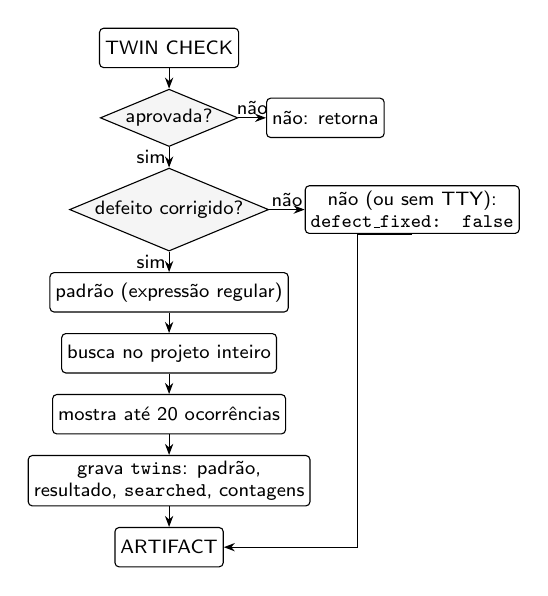
\begin{tikzpicture}[
  font=\sffamily\scriptsize, >={Stealth[length=4pt]},
  proc/.style={draw, thin, rounded corners=1.5pt, align=center, fill=white, minimum height=0.5cm, inner sep=2pt},
  dec/.style={draw, thin, diamond, aspect=2.4, align=center, fill=black!4, inner sep=0.5pt, font=\sffamily\scriptsize},
  nota/.style={font=\sffamily\scriptsize, align=center, text=black!80},
  lbl/.style={font=\sffamily\scriptsize, inner sep=1pt}
]
\node[proc] (a) {TWIN CHECK};
\node[dec, below=0.26cm of a] (ap) {aprovada?};
\node[proc, right=0.35cm of ap] (r1) {não: retorna};
\node[dec, below=0.26cm of ap] (df) {defeito corrigido?};
\node[proc, right=0.45cm of df] (r2) {não (ou sem TTY):\\ \texttt{defect\_fixed: false}};
\node[proc, below=0.26cm of df] (pat) {padrão (expressão regular)};
\node[proc, below=0.26cm of pat] (sr) {busca no projeto inteiro};
\node[proc, below=0.26cm of sr] (sh) {mostra até 20 ocorrências};
\node[proc, below=0.26cm of sh] (rec) {grava \texttt{twins}: padrão,\\ resultado, \texttt{searched}, contagens};
\node[proc, below=0.26cm of rec] (n) {ARTIFACT};
\coordinate (chan) at ($(rec.east)+(0.60,0)$);
\draw[->] (a) -- (ap);
\draw[->] (ap) -- node[lbl,above]{não} (r1);
\draw[->] (ap) -- node[lbl,left]{sim} (df);
\draw[->] (df) -- node[lbl,above]{não} (r2);
\draw[->] (df) -- node[lbl,left]{sim} (pat);
\draw[->] (pat) -- (sr);
\draw[->] (sr) -- (sh);
\draw[->] (sh) -- (rec);
\draw[->] (rec) -- (n);
\draw[->] (r2.south) -- (r2.south -| chan) -- (n -| chan) -- (n.east);
\end{tikzpicture}
\end{document}
